\documentclass[9pt,twoside]{pnas-new}
% Use the lineno option to display guide line numbers if required.

\articletype{First report}%%%% Article topic/classification

\templatetype{pnasmathematics} % Choose template
% {pnasresearcharticle} = Template for a two-column research article
% {pnasmathematics} = Template for a one-column mathematics article
% {pnasinvited} = Template for a PNAS invited submission
%\onecolumn

\begin{document}

\title{Speaking Out: Critical Mass in Group Discussions with Heterogeneous Agents}

\author[a]{Lana Tkalčič}
\author[a]{Matjaž Kranjčec}
\affil[a]{University of Ljubljana, Faculty of Computer and Information Science}

%\authorcontributions{...}   % lahko izbrišeš ali izpolniš
\correspondingauthor{E-mail: lt80473@student.uni-lj.si, mk92169@student.uni-lj.si}


\keywords{agent-based model $|$ critical mass $|$ social conventions $|$ opinion dynamics}

\begin{abstract}
How many people have to speak out in a group discussion before the majority adopts their view? The theory of critical mass states that a committed minority can overturn an established social convention once it exceeds a threshold size. Experiments and models place this threshold anywhere from a few percent to 40\% of the population, depending on how individuals interact and how readily they change their minds. These models, however, treat all individuals as identical, although people differ in their willingness to voice an opinion, in their susceptibility to social pressure and in their tolerance of disagreement. In this first report, we review the relevant concepts and models and reimplement the higher-order naming game of Iacopini \emph{et al.}, in which a committed minority interacts with the rest of the population in groups of three. Agent-based simulations agree with the mean-field description and recover the published behaviour: the critical mass is about 12.5\% when agreement always succeeds, falls to about 3\% when agents only partly yield to the group, and when agents are too reluctant to yield, no single convention prevails. Finally, we outline how we will extend the model with agents that differ in boldness, conformity, tolerance and strength of belief.
\end{abstract}

\maketitle
\ifthenelse{\boolean{shortarticle}}{\ifthenelse{\boolean{singlecolumn}}{\abscontentformatted}{\abscontent}}{}
\firstpage[1]{8}

\section{Introduction}

Social conventions, such as the words we use or the opinions we are willing to
voice, are usually very stable, yet they sometimes change abruptly. A common
explanation is the existence of a \emph{tipping point}: once the number of
people who openly support an alternative exceeds a \emph{critical mass}, the
rest of the population follows. The idea goes back to threshold models of
collective behaviour~\cite{granovetter1978threshold} and to studies of
minorities in organisations, which argued that a minority of less than about
15\% is treated as a token, whereas a larger one can begin to shape the culture
of the group~\cite{kanter1977some}. Centola
\emph{et al.}~\cite{centola2018experimental} tested the idea in an online
experiment: groups first agreed on a name, then a committed minority was
introduced, and the established convention was overturned once the minority
reached about 25\% of the group.

\paragraph*{The naming game and committed minorities}
The simplest model of how a convention emerges is the naming game
(NG)~\cite{steels1995self,baronchelli2006sharp}. Each agent keeps a list of
names, its \emph{vocabulary}, for the same object. In each interaction, a
speaker utters one of its names to a listener. If the listener already knows
the name, both keep only that name; otherwise, the listener adds it to its
vocabulary. In a well-mixed population, this local rule always leads to global
agreement on a single name~\cite{baronchelli2006sharp}.
Baronchelli \emph{et al.}~\cite{baronchelli2007nonequilibrium} introduced a
parameter $\beta$, the probability that a successful interaction actually ends
in agreement; for $\beta<1/3$, consensus is lost and two names coexist.
Xie \emph{et al.}~\cite{xie2011social} added a fraction $p$ of
\emph{committed} agents, who hold one name and never change it. Such a
minority overturns a convention held by everyone else only if $p$ exceeds about
10\%, and the threshold rises to as much as 40\% when commitment is
weaker~\cite{niu2017impact}. These and related models of social dynamics are
reviewed in~\cite{castellano2009statistical}.

\paragraph*{Group interactions}
Real discussions rarely take place in pairs. Interactions that involve several
people at once are naturally described as hyperedges of a
hypergraph~\cite{battiston2020networks}. Iacopini
\emph{et al.}~\cite{iacopini2022group}, the starting point of our project,
extended the NG with committed minorities to group interactions. In their
model, a speaker addresses a whole group, and the group converges on the
spoken name only if all listeners already know it. Their central result is
that group interactions can strongly lower the critical mass: when agents are
only partly susceptible to social influence (intermediate $\beta$), a committed
minority of a few percent is enough to overturn the convention, far below the
10\% of the pairwise model. They also showed that the outcome depends on the
size of the groups in a non-monotonic way.

\paragraph*{Bounded confidence and the spiral of silence}
Two further lines of research motivate our extensions. In bounded-confidence
models~\cite{deffuant2000mixing,hegselmann2002opinion}, two agents influence
each other only if their opinions are sufficiently close. This confidence bound
acts as a \emph{tolerance} and determines whether the population reaches
consensus or splits into clusters. The theory of the spiral of
silence~\cite{noelleneumann1974spiral} states that people who believe their
opinion to be in the minority tend to stay silent, which makes that opinion
appear even less popular. The willingness to speak out differs between
individuals and can be measured with surveys~\cite{hayes2005willingness}, and
recent models show how the gap between private and expressed opinions distorts
what a population perceives as the majority
view~\cite{gaisbauer2020dynamics,vilone2023modelling}. Classic experiments
further show that individuals differ in how strongly they yield to a
majority~\cite{asch1956studies} and that a \emph{consistent} minority can shift
the judgement of the majority~\cite{moscovici1969influence}.

\paragraph*{Our approach}
In all the critical-mass models above, every non-committed agent follows the
same rule with the same parameters. We ask how the share of committed speakers
needed to shift the majority changes when individuals differ in their
\emph{boldness} (how likely they are to speak), \emph{conformity} (how readily
they give up their view), \emph{tolerance} (how much disagreement they accept)
and \emph{belief strength}. In this first report, we (i) review the relevant
concepts and models, (ii) reimplement the baseline model of Iacopini
\emph{et al.}~\cite{iacopini2022group} for groups of three and compare it with
their mean-field description, and (iii) outline how we will introduce agents
with heterogeneous traits, parameterised with survey data.

\section{Methods}

\subsection{Baseline model}
We follow the model of Iacopini \emph{et al.}~\cite{iacopini2022group} on a
homogeneously mixed population of $N$ agents. Each agent holds name A, name B,
or both (AB). A fraction $p$ of the agents is committed to A and never changes
its vocabulary. All other agents initially hold only B, so B is the established
convention. In each interaction, three distinct agents are drawn at random. One
of them, chosen at random, is the speaker and utters a name drawn uniformly from
its vocabulary; the other two are listeners.

Agreement follows the \emph{unanimity} rule of~\cite{iacopini2022group}: it is
possible only if both listeners already know the spoken name. In that case, with
probability $\beta$, all non-committed members of the group discard every other
name and keep only the spoken one; with probability $1-\beta$, nothing changes.
If agreement is not possible, each listener that did not know the name adds it
to its vocabulary. The parameter $\beta$ thus measures how readily agents give
up their view for the sake of the group. When the group is reduced to a pair and
$\beta=1$, the model reduces to the NG with committed agents of Xie
\emph{et al.}~\cite{xie2011social}. Time $t$ is measured in units of $N$
interactions, so that on average every agent takes part in three interactions
per unit of time.

\subsection{Mean-field description}
Let $n_A$, $n_B$ and $n_{AB}$ denote the fractions of agents that are not
committed and hold only A, only B, or both names, so that
$n_A+n_B+n_{AB}+p=1$. In a large, well-mixed population, the three members of a
group can be treated as independent. A speaker utters A with probability
$P_A=n_A+p+n_{AB}/2$ and B with probability $P_B=n_B+n_{AB}/2$, and a listener
knows A with probability $q_A=1-n_B$ and B with probability $q_B=1-n_A-p$.
Summing the expected changes over all possible groups gives, up to a constant
rescaling of time,
\begin{align}
\frac{dn_A}{dt} &= \beta\, n_{AB}\left(\tfrac12\, q_A^{2} + 2P_A\, q_A\right) - 2P_B\, n_A, \label{eq:mfA}\\
\frac{dn_B}{dt} &= \beta\, n_{AB}\left(\tfrac12\, q_B^{2} + 2P_B\, q_B\right) - 2P_A\, n_B. \label{eq:mfB}
\end{align}
In Eq.~\ref{eq:mfA}, the first term describes an AB speaker whose name A is
accepted by both listeners, the second an AB listener who adopts A together with
the rest of the group, and the last an A agent who hears B and learns it.
Eq.~\ref{eq:mfB} is obtained by exchanging A and B, with the committed agents
counted among the holders of A. Expanded, Eqs.~\ref{eq:mfA}--\ref{eq:mfB} are
equivalent to Eq.~1 of~\cite{iacopini2022group}.

We integrate the equations numerically from $n_A=n_{AB}=0$ and $n_B=1-p$ until
they reach a stationary state. As the order parameter we use the stationary
fraction of agents that hold only A, including the committed ones,
$n_A^{*}+p$. We define the critical mass $p_c(\beta)$ as the smallest $p$ for
which $n_A^{*}+p>1/2$, and we locate it by bisection.

\subsection{Simulations}
The agent-based model is implemented in Python with the Mesa
framework~\cite{kazil2020utilizing}. We verified that its update rule is
identical to the reference implementation of~\cite{iacopini2022group}. We
simulate $N=1000$ agents for $\beta\in\{0.3, 0.4, 0.7, 1\}$ and for $p$ from
0 to 0.2 in steps of 0.01, with ten independent runs for each pair of
parameters. Every run lasts until all agents hold the same name or until
$t=1000$. We record $n_A+p$, $n_B$ and $n_{AB}$ once per unit of time. If a run
reaches consensus, we take the final value of $n_A+p$; otherwise, we average it
over the last 100 units of time, which removes the fluctuations of the
coexistence state. The code and the scripts that reproduce all figures are
available in our
repository.\footnote{\url{https://github.com/Lankovski12/Collective_behavior-Group_G}}

\subsection{Planned extensions}
Our main contribution will be to replace identical agents with agents that
carry individual traits:
\begin{itemize}
\item \textbf{Boldness} $b_i\in[0,1]$: the probability that agent $i$ speaks
when it is chosen as the speaker. A silent agent does not reveal its name, so
its view remains hidden, as in the spiral of
silence~\cite{noelleneumann1974spiral}.
\item \textbf{Conformity} $c_i\in[0,1]$: an individual version of $\beta$, the
probability that agent $i$ adopts the name the group has agreed on.
\item \textbf{Tolerance} $\tau_i$: the largest fraction of listeners who may
not know the spoken name for agent $i$ still to accept the agreement. The value
$\tau_i=0$ recovers the unanimity rule, while larger values move towards the
union rule of~\cite{iacopini2022group}, analogous to the confidence bound
in~\cite{deffuant2000mixing}.
\item \textbf{Belief strength} $s_i$: a graded resistance to change that
replaces the binary distinction between committed and non-committed agents, in
the spirit of~\cite{niu2017impact}.
\end{itemize}
The traits will be drawn from distributions estimated from survey data on
five-factor personality traits~\cite{mccrae1992introduction} and on the
willingness to self-censor~\cite{hayes2005willingness}. For each setting, we
will measure how the critical mass $p_c$ depends on the mean and the spread of
each trait, and whether it matters \emph{which} agents are committed, for
example the boldest ones.

\section{Results}

\begin{figure}[H]
\centering
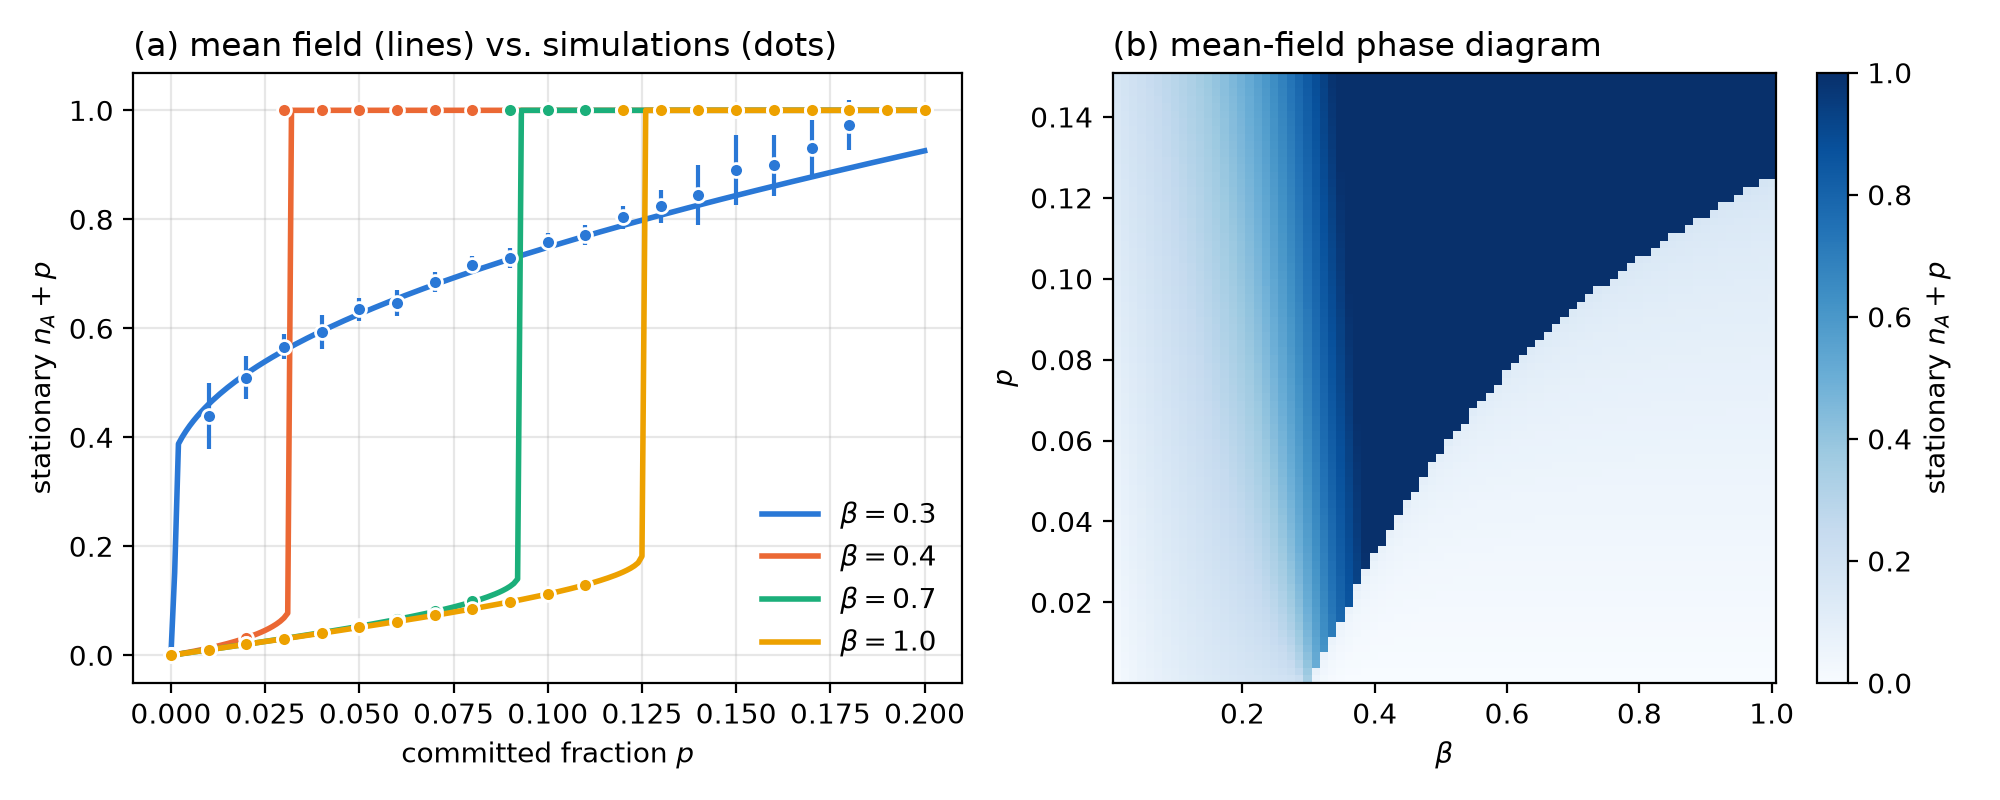
\includegraphics[width=\linewidth]{figures/fig1.png}
\caption{Baseline model with groups of three under the unanimity rule.
(a) Stationary fraction of agents holding only A, $n_A^{*}+p$, as a function
of the committed fraction $p$. Lines show the mean-field solution of
Eqs.~\ref{eq:mfA}--\ref{eq:mfB}; dots show the mean over ten agent-based
simulations with $N=1000$, and error bars one standard deviation.
(b) Mean-field phase diagram of $n_A^{*}+p$ in the $(\beta,p)$ plane. In the
dark region the committed minority overturns the convention, in the light
region below it the convention B survives, and for $\beta\lesssim1/3$ the two
names coexist.}
\label{fig:baseline}
\end{figure}

\paragraph*{Mean-field solution}
The mean-field phase diagram (Fig.~\ref{fig:baseline}b) shows two distinct
regimes. For $\beta\lesssim1/3$, the population never reaches consensus: a large
fraction of agents keeps both names, and $n_A^{*}+p$ grows continuously with
$p$. For $\beta\gtrsim1/3$, the stationary state changes abruptly. Below a
critical value $p_c(\beta)$, the committed minority converts only a few agents
and B remains the convention; above it, the whole population adopts A. The
critical mass grows with $\beta$ (Table~\ref{tab:pc}): a minority of about 3\%
suffices at $\beta=0.4$, whereas about 12.5\% is needed at $\beta=1$. A
committed minority is therefore most effective when agents are only moderately
susceptible to social influence, as reported by Iacopini
\emph{et al.}~\cite{iacopini2022group}. For comparison, the pairwise NG with
$\beta=1$ has a critical mass of about 10\%~\cite{xie2011social}. At
$\beta=0.3$, the condition $n_A^{*}+p>1/2$ is met already for $p\approx1.7\%$,
but here it reflects a mixed state rather than a switch to a new convention.

\begin{table}[t]
\centering
\caption{Critical mass for groups of three. The mean-field value $p_c$ was
obtained by bisection; the simulation interval gives the largest $p$ on our
grid at which all runs kept convention B and the smallest $p$ at which all runs
reached consensus on A.}
\label{tab:pc}
\begin{tabular}{ccc}
\hline
$\beta$ & $p_c$ (mean field) & transition in simulations \\
\hline
0.4 & 0.032 & $0.02$--$0.03$ \\
0.7 & 0.092 & $0.08$--$0.09$ \\
1.0 & 0.125 & $0.11$--$0.12$ \\
\hline
\end{tabular}
\end{table}

\paragraph*{Agent-based simulations}
The simulations reproduce the mean-field results closely
(Fig.~\ref{fig:baseline}a). For $\beta\ge0.4$ and $p<p_c$, the simulated
$n_A+p$ differs from the mean-field value by less than $0.005$, and the spread
between runs is negligible. Above $p_c$, all ten runs end in consensus on A.
In the coexistence regime ($\beta=0.3$), the simulations follow the mean-field
curve to within about $0.02$ up to $p\approx0.14$, with a larger spread between
runs.

The simulations deviate from the mean-field description in two ways, both due
to the finite size of the population. First, the transition occurs slightly
below the mean-field critical mass: at $p=0.03$, $0.09$ and $0.12$, which lie
0.002--0.005 below $p_c$, all runs reached consensus on A
(Table~\ref{tab:pc}). Close to $p_c$, the state dominated by B is only weakly
stable, and random fluctuations are enough to push a population of 1000 agents
across the threshold within the simulated time. Second, at $\beta=0.3$ and
$p\gtrsim0.15$, the simulated values lie above the mean-field curve, and for
$p\ge0.19$ all runs end with every agent holding A. In this regime, only a few
agents hold B alone; they can disappear by chance, and since consensus on A is
an absorbing state, the population cannot return to coexistence.

\section{Discussion}

We reimplemented the higher-order naming game of Iacopini
\emph{et al.}~\cite{iacopini2022group} for groups of three and verified it in
two independent ways: the update rule matches the reference implementation,
and the simulations agree with the mean-field equations. The baseline
reproduces the main finding of the original study. The critical mass depends
strongly on how readily agents yield to the group: it is smallest for $\beta$
just above $1/3$, where a committed minority of about 3\% overturns the
convention, and increases to about 12.5\% when agreement always succeeds.
Agents who are open to influence but do not give up their view at once thus
make a population easier to tip. When they are too reluctant
($\beta\lesssim1/3$), the population no longer converges on any single
convention.

Our results also show where the mean-field description reaches its limits. In a
population of 1000 agents, the critical mass is slightly lower than predicted,
because fluctuations allow the system to escape from a weakly stable state, and
in the coexistence regime the minority name can be lost by chance. Both effects
are expected to weaken as $N$ grows.

The baseline has several limitations. We considered only a homogeneously mixed
population, groups of exactly three and the unanimity rule, whereas Iacopini
\emph{et al.}~\cite{iacopini2022group} also studied larger groups, the union
rule and empirical hypergraphs. We used ten runs per parameter pair and a
coarse grid in $p$, so the transition in the simulations is located only to
within $0.01$. Most importantly, all non-committed agents are identical and
differ only in their vocabulary.

This last limitation is the focus of our future work. Because the critical mass
depends so strongly on $\beta$, we expect the spread of individual conformity
$c_i$ around the same mean to change the outcome, for example when only a
fraction of the population lies above $1/3$. Boldness will reduce the number of
names actually spoken, so that the views of silent agents remain invisible to
others, while tolerance and belief strength will soften the agreement rule and
the binary notion of commitment. In the next stage, we will implement these
traits one at a time, starting with conformity, compare each variant with the
baseline presented here, and choose a survey dataset from which to estimate the
trait distributions.

\acknow{LT mostly wrote the report and fixed some minor problems with the code. MK reimplemented the original article then reviewed and edited the report.}

\showacknow{}

\bibliography{references}

\end{document}